\documentclass[a4paper,11pt]{report}

%%%%%%%%%%%%%%%%%%%%%%%%%%%%%%%%%% Packages %%%%%%%%%%%%%%%%%%%%%%%%%%%%%%%%%%

\usepackage[utf8]{inputenc}
\usepackage{graphicx}
\usepackage[T1]{fontenc}
\usepackage[english]{babel}
\usepackage{float}
\usepackage{amsmath, amssymb}
\usepackage{geometry}
\usepackage{siunitx}
\geometry{margin=2.5cm}
\usepackage{hyperref}

\newcommand{\HRule}{\rule{\linewidth}{0.5mm}}

\begin{document}


%%%%%%%%%%%%%%%%%%%%%%%%%%%%%%%%%% Title Page %%%%%%%%%%%%%%%%%%%%%%%%%%%%%%%%%%

\begin{center}

% Upper part of the page. The '~' is needed because only works if a paragraph has started.
\includegraphics[width=0.55\textwidth]{Image/logo.png}~\\[1cm]

\textsc{\LARGE Telecom Physique Strasbourg}\\[1.5cm]

\textsc{\Large }\\[0.5cm]

% Title
\HRule \\[0.4cm]

{\huge Silicon Fiber-to-Chip Grating Coupler \bfseries  \\[0.4cm] }

\HRule \\[1.5cm]

\begin{minipage}{0.4\textwidth}
\begin{flushleft} \large
\emph{Author:}\\
Nolan \textsc{LE TYRANT}\\

\end{flushleft}
\end{minipage}
\begin{minipage}{0.4\textwidth}
\end{minipage}

\vfill

% Bottom of the page
{\large \today}

\end{center}
\thispagestyle{empty}

\tableofcontents
%%%%%%%%%%%%%%%%%%%%%%%%%%%%%%%%%% Chapitre 1 : Introduction %%%%%%%%%%%%%%%%%%%%%%%%%%%%%%%%%%

\chapter{Introduction}

\section{Context and objectives}

Grating couplers are key components of silicon-integrated photonics: they allow light from an optical fiber, arriving in free space, to be efficiently coupled into the guided mode of a photonic circuit on chip. This type of component is, for example, used for the optical interfacing of integrated circuits in silicon photonics.

The objective of this project is to design, simulate, and optimize a silicon fiber-to-chip grating coupler, using the FDTD (Finite-Difference Time-Domain) method, and to maximize its coupling efficiency at a wavelength of 1{,}55~\textmu m (standard telecom wavelength). More precisely, this work aims to:

\begin{itemize}
    \item establish an initial analytical estimate of the grating geometry, from the phase-matching condition 
    \item implement an FDTD simulation of the device, with a source representing the mode of a single-mode optical fiber 
    \item numerically validate the reliability of the results obtained, by identifying and correcting artifacts specific to the FDTD method 
    \item optimize the geometric parameters of the grating (period, duty cycle) through parametric sweeps, then through a gradient-based optimization method 
    \item discuss the limitations of the approach and possible avenues for improvement
\end{itemize}

\section{General approach}

The approach followed combines an analytical method with numerical simulation. A first estimate of the grating period is obtained analytically (chapter~\ref{ch:theorie}), from a simplified model of the guided mode's effective index. 

Since the very first simulation results revealed inconsistencies due to spatial discretization artifacts, a numerical validation step (chapter~\ref{ch:validation}) was necessary before the optimization results could be interpreted. This validation includes a study of the spatial alignment between the computational grid and the device, as well as a resolution convergence study.

Once the method was validated, the grating's geometric parameters (period $\Lambda$ and duty cycle $gdc$) were first optimized manually through a parametric sweep, then through a gradient-based optimization method (chapter~\ref{ch:resultats}).

\section{Report outline}

Chapter~\ref{ch:theorie} presents the theoretical model of grating coupling and the initial analytical estimate of the period. Chapter~\ref{ch:numerique} details the implementation of the FDTD simulation and the physical parameters used. Chapter~\ref{ch:validation} presents the numerical validation process that established the reliability of the results. Chapter~\ref{ch:resultats} presents the optimization results, obtained through manual sweeping and then through the gradient method. Finally, the conclusion revisits the limitations of the work carried out and proposes avenues for improvement.

%%%%%%%%%%%%%%%%%%%%%%%%%%%%%%%%%% Chapitre 2: Théorie %%%%%%%%%%%%%%%%%%%%%%%%%%%%%%%%%%
\chapter{Theoretical model}
\label{ch:theorie}

\section{Device description}
The simulated device consists of an incident beam (assumed to arrive via an optical fiber) at an angle $\theta$ onto a periodic grating of teeth, followed by a guided mode. The device schematic is as follows:
\begin{figure}[h]
    \centering
    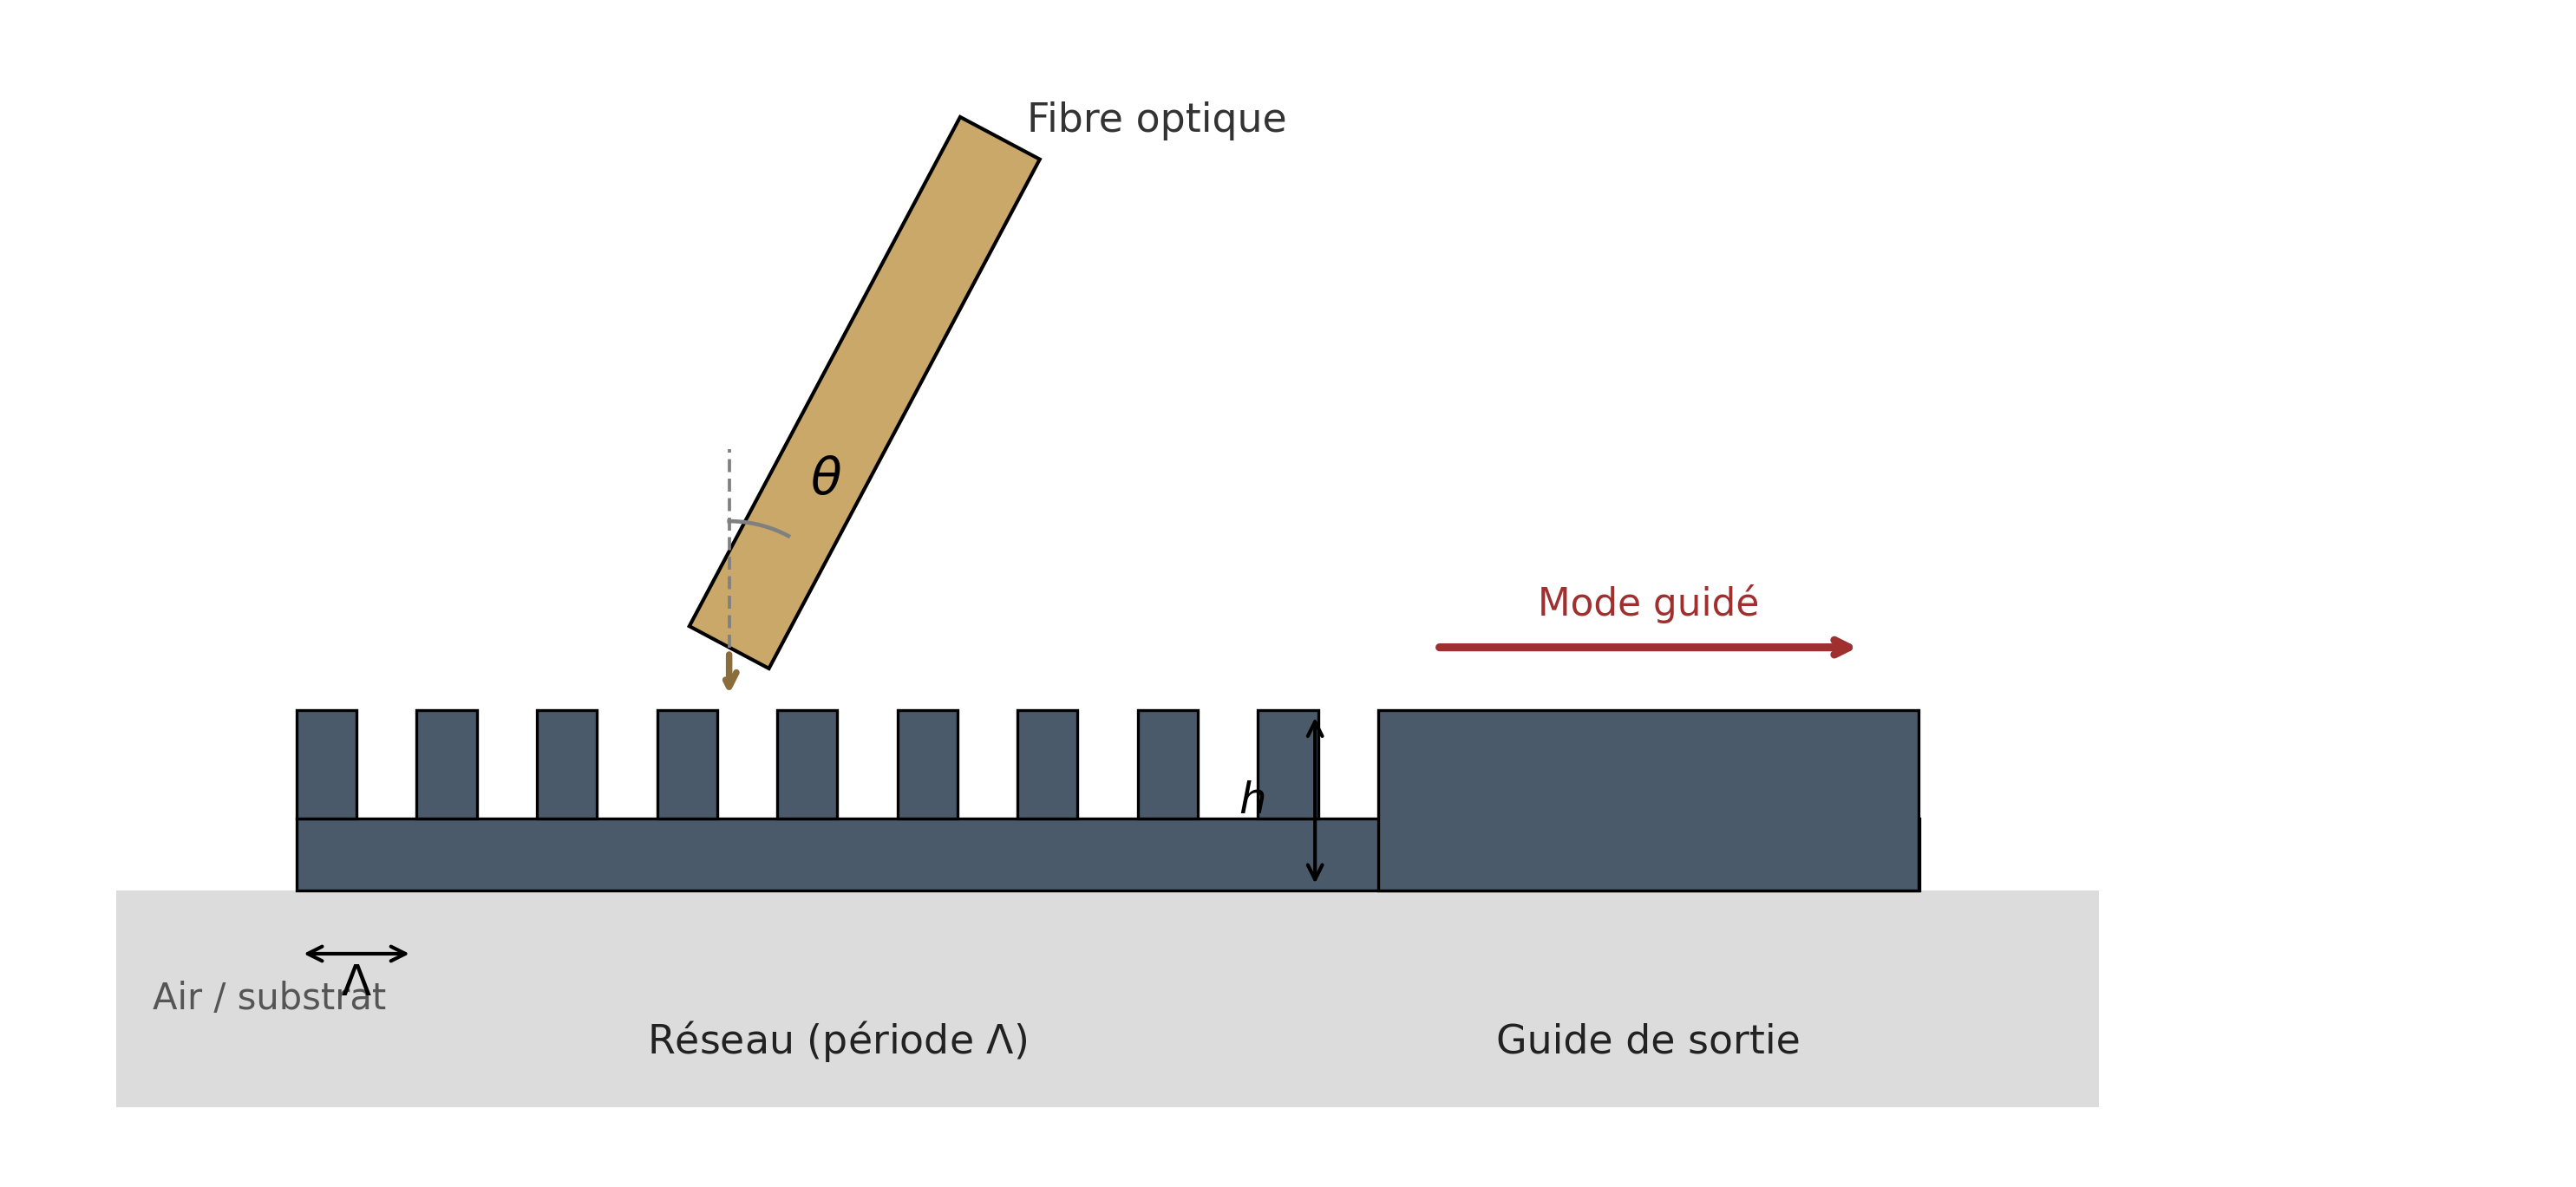
\includegraphics[width=0.85\linewidth]{Image/shema.png}
    \caption{Schematic of the modeled device: tilted optical fiber, diffraction grating, output waveguide}
    \label{fig:schema_dispositif}
\end{figure}

\section{Phase-matching condition}

The grating must redirect the incident light, arriving in free space, toward the guided mode of the silicon. This condition is formulated as a constructive interference condition between the successive contributions of the grating teeth, analogous to the classical condition for bright fringes in optics, where the path difference between two paths must be an integer multiple of the wavelength.

\subsection*{Calculation of the two optical paths}

Consider two consecutive teeth of the grating, separated by the period $\Lambda$ (figure~\ref{fig:diff_marche}).

\begin{figure}[h]
    \centering
    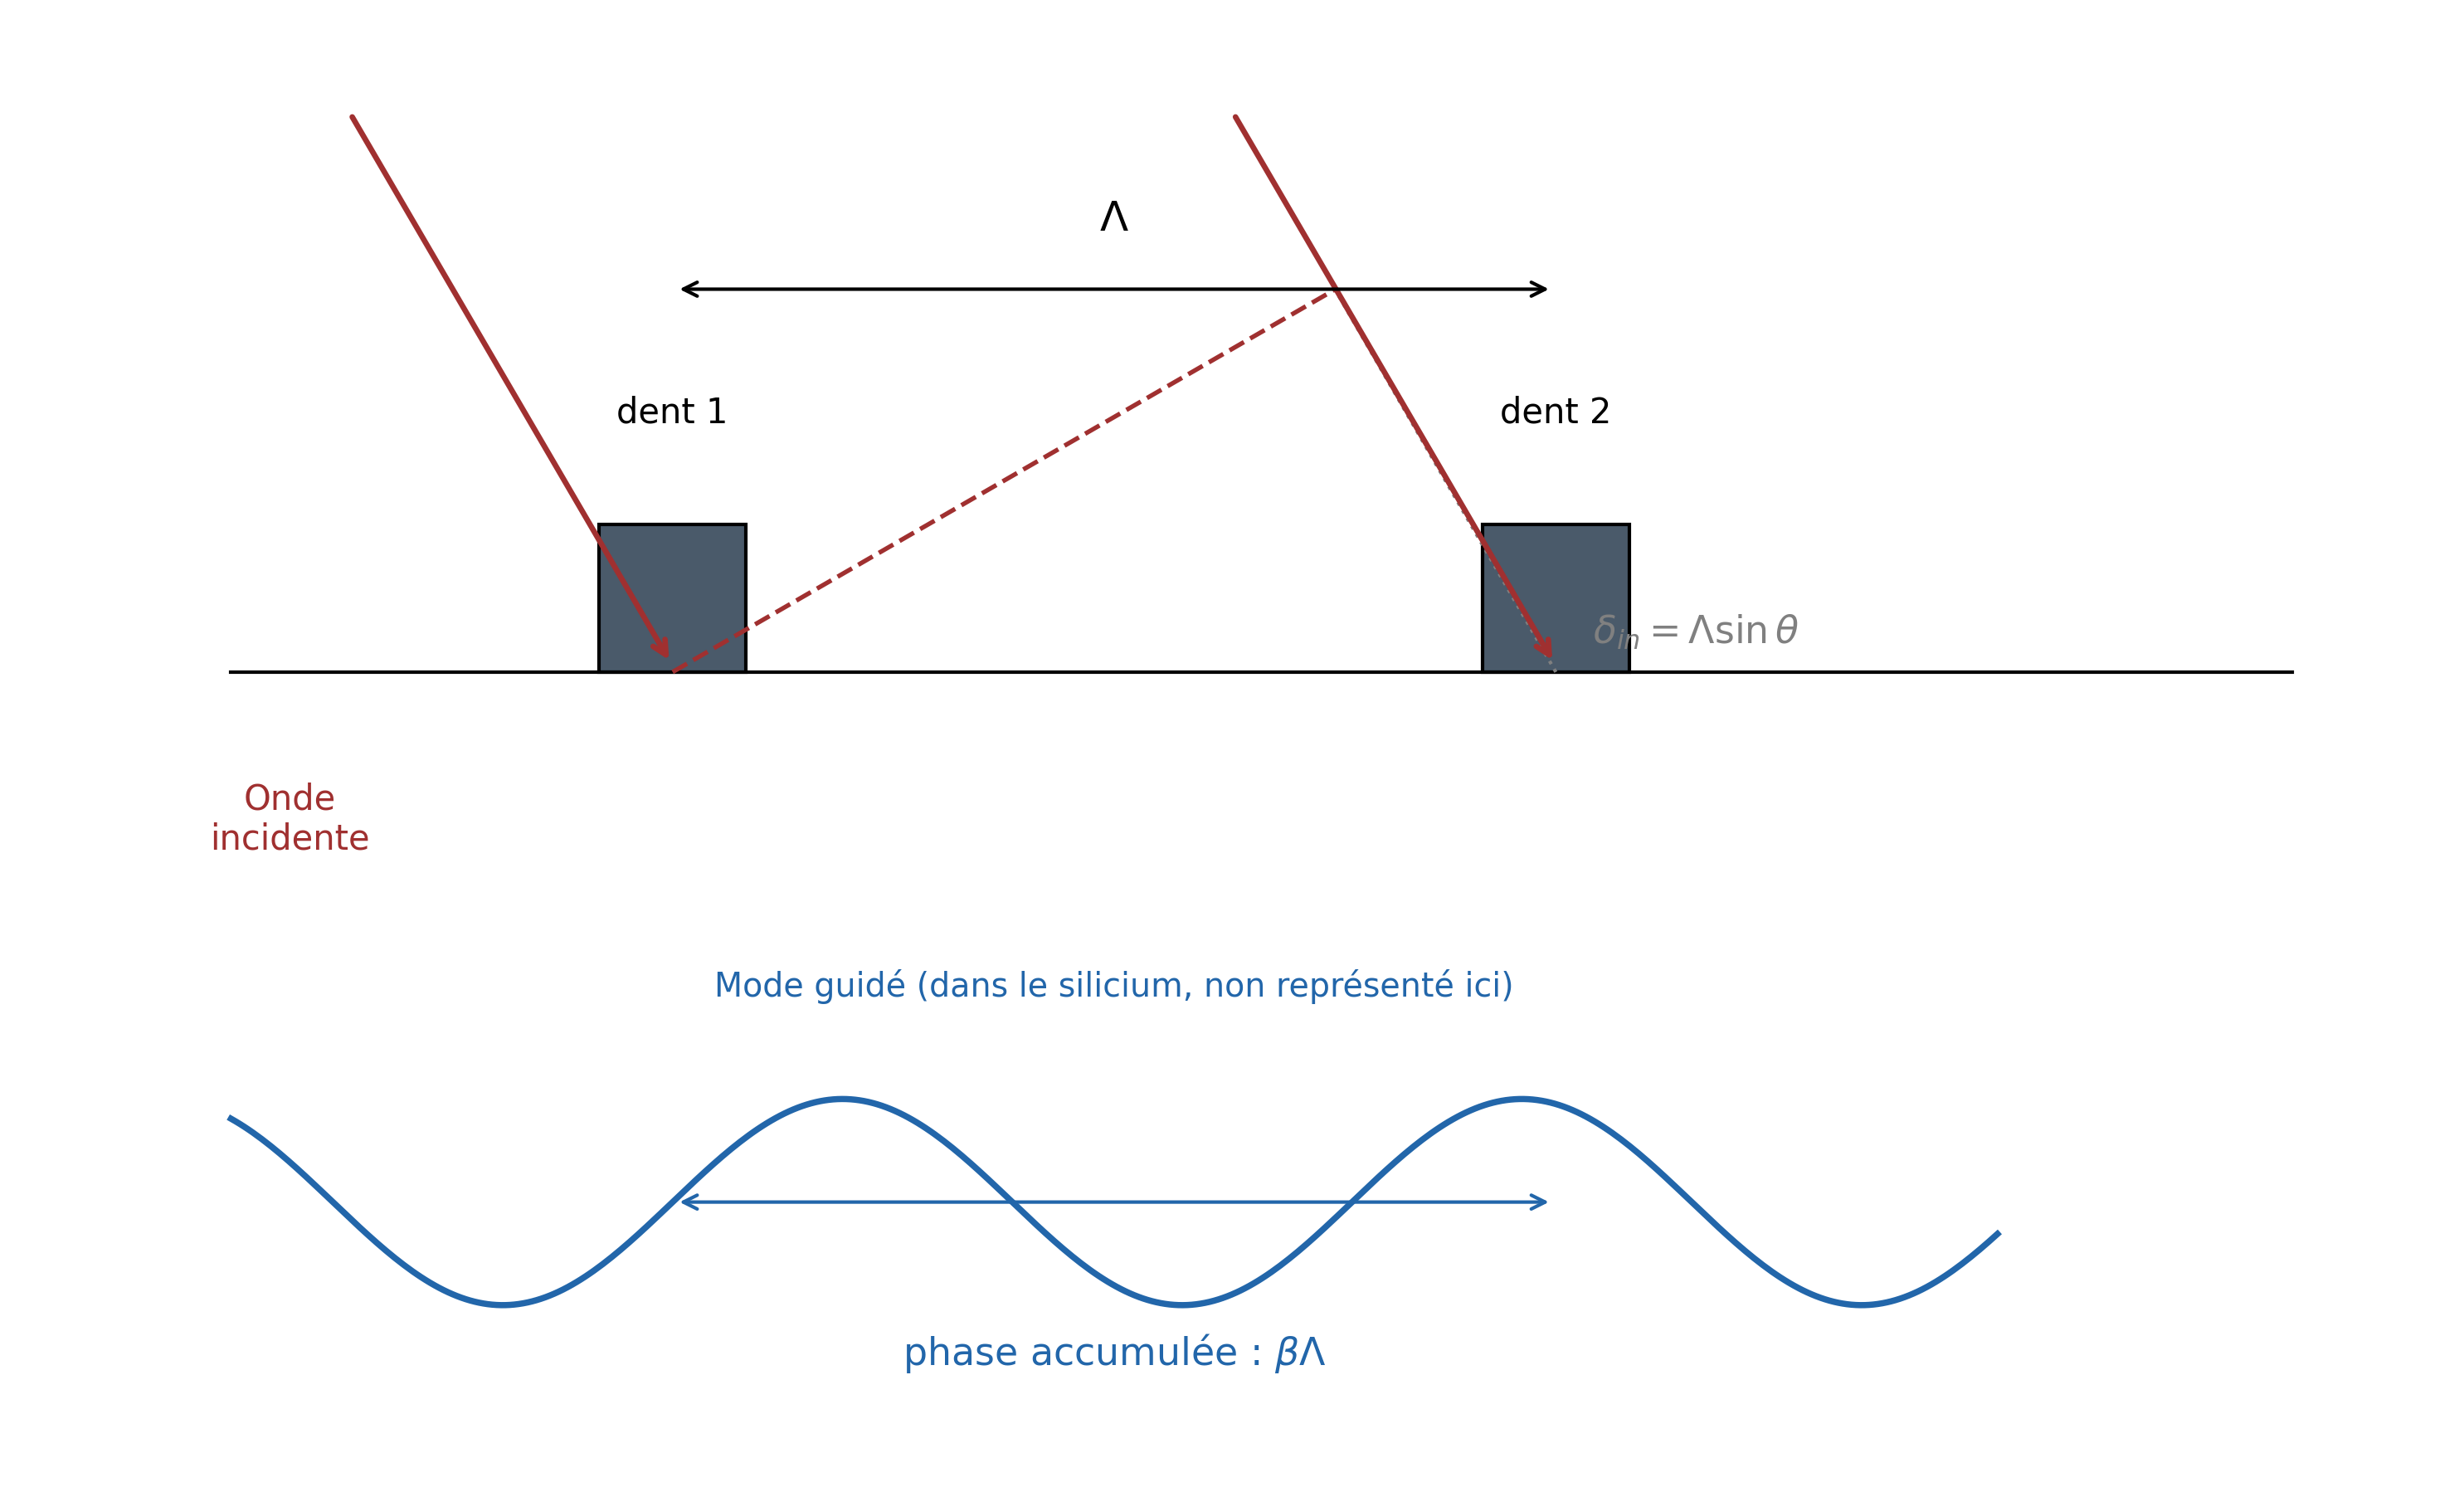
\includegraphics[width=0.85\linewidth]{Image/accord_de_phase.png}
    \caption{Path difference between two consecutive grating teeth: $\delta_{in}$ on the incident-wave side, $\delta_{guide}$ on the guided-mode side}
    \label{fig:diff_marche}
\end{figure}

\paragraph{Optical path on the incident-wave side.} The incident wave, arriving at an angle $\theta$ with respect to the normal, reaches the second tooth with a geometric delay relative to the first. This delay corresponds to an additional propagation distance in the incident medium (air, index $n_{clad}$):
\begin{equation}
\delta_{in} = n_{clad}\cdot\Lambda\sin\theta
\end{equation}

\paragraph{Optical path on the guided-mode side.} The guided mode, once excited, propagates in the waveguide with an effective index $n_{eff}$ (computed in section~\ref{sec:calcul_neff}). The optical path it travels over this same distance $\Lambda$ is:
\begin{equation}
\delta_{guide} = n_{eff}\cdot\Lambda
\end{equation}

\subsection*{Constructive interference condition}

For the successive contributions of the teeth to add up constructively in the guided mode, the path difference between these two optical paths must be an integer multiple $m$ of the wavelength $\lambda$:

\begin{equation}
\delta_{guide} - \delta_{in} = m\lambda
\label{eq:diff_marche}
\end{equation}
Substituting, we thus obtain:
\begin{equation}
n_{eff}\cdot\Lambda - n_{clad}\cdot\Lambda\sin\theta = m\lambda
\label{eq:accord_phase}
\end{equation}

This equation is the phase-matching condition of the \textit{grating coupler}. It expresses that the grating must exactly compensate, period after period, the difference between the phase accumulated by the incident wave and the phase that the guided mode would accumulate over the same distance (an integer multiple of $2\pi$ not affecting the interference, which justifies the presence of the integer $m$, the diffraction order).

Thus, we obtain the following formula for the period:
\begin{equation}
\boxed{\Lambda = \frac{m\lambda}{n_{eff} - n_{clad}\sin\theta}}
\label{eq:lambda_theorique}
\end{equation}

\section{Choice of starting values}
For a first estimate (standard silicon photonics values):
\begin{itemize}
    \item $\lambda = 1{,}55~\mu\text{m}$: the standard telecom wavelength 
    \item $h = 220 ~\text{nm}$ (standard thickness for silicon-on-insulator chips)
    \item $\theta = 10^\circ$: angle of the incident beam coming from the optical fiber
    \item $m = 1$: the first diffraction order
    \item $n_{\text{clad}} = 1$ (air)
    \item $n_{\text{core}} = \sqrt{12} \approx 3{,}464$ (silicon)

\end{itemize}

\section{Calculation No. 1: Effective permittivity model}
\label{sec:calcul_neff}

\subsection*{Setting up the equation}

Taking a wave field of the form:
\begin{equation}
\psi(y) \cdot e^{i (\beta x - \omega t)}
\end{equation}
where $\beta$ is the propagation constant of the guided mode (related to the effective index by $\beta=n_{\text{eff}}\cdot k_0$, with $k_0=2\pi/\lambda$ the vacuum wavevector), and using Maxwell-Ampère's and Maxwell-Faraday's equations, we obtain the transverse Helmholtz equation:
\begin{equation}
\frac{\text{d}^2\psi}{\text{d}y^2} + (n^2 k_0^2 - \beta^2) \psi = 0
\end{equation}

In the core ($n = n_{\text{core}}$), to have a guided mode (i.e., a profile that oscillates in the core), we need $n_{\text{core}} \cdot k_0 > \beta$ (sinusoidal solution), so we have:
\begin{equation}
k_y^2 = n_{\text{core}}^2 \cdot k_0^2 - \beta^2 > 0
\end{equation}
($k_y$ denoting here the transverse propagation constant along the $y$ axis, not to be confused with a possible component along $x$, the grating's propagation direction used elsewhere in this report)

In the cladding ($n = n_{\text{clad}}$), on the contrary $\beta > n_{\text{clad}} \cdot k_0$ (guiding condition: the wave is "too slow" to propagate freely in the cladding, so it becomes evanescent there), so we have:
\begin{equation}
\gamma^2 = \beta^2 - n_{\text{clad}}^2 \cdot k_0^2 > 0
\end{equation}

Hence:
\begin{equation}
k_y^2 + \gamma^2 = (n_{\text{core}}^2 \cdot k_0^2 - \beta^2) + (\beta^2 - n_{\text{clad}}^2 \cdot k_0^2) = (n_{\text{core}}^2 - n_{\text{clad}}^2) \cdot k_0^2
\end{equation}

From the differential equations we deduce the following forms in the cladding and the core:
\begin{itemize}
    \item \textbf{Core} ($|y| < a$): $\psi(y) = A \cdot \cos(k_y \cdot y)$
    \item \textbf{Cladding} ($y > a$): $\psi(y) = B \cdot \exp(-\gamma (y-a))$
\end{itemize}

Here we use the physical conditions from Maxwell's equations: the electric field and its normal derivative (related to the tangential magnetic field) must be continuous at the core/cladding interface, otherwise the continuity of $H_{\text{tangential}}$, imposed by Maxwell's equations in the absence of a surface current, would be violated.

\vspace{0.5em}
\noindent \textbf{Continuity of $\psi$ at $y=a$:}
\begin{equation}
A \cdot \cos(k_y \cdot a) = B
\end{equation}

\noindent \textbf{Continuity of $\frac{\text{d}\psi}{\text{d}y}$ at $y=a$:}
\begin{equation}
-A \cdot k_y \cdot \sin(k_y \cdot a) = -B \cdot \gamma
\end{equation}

Dividing the second equation by the first:
\begin{equation}
\frac{k_y \cdot \sin(k_y \cdot a)}{\cos(k_y \cdot a)} = \gamma \quad \implies \quad k_y \cdot \tan(k_y \cdot a) = \gamma
\label{eq:transcendante_ch1}
\end{equation}

\subsection*{Validation of the solving method}

Before applying this equation to the etched geometry, the solving method (root finding via Brent's method) was validated on the simple case of a full, non-etched waveguide, by comparing it to an independent FDTD simulation of this same waveguide. The center frequency found in this simulation matches the design wavelength of $1{,}55~\mu\text{m}$ well. The dominant propagation wavevector obtained is $\beta \approx 1{,}776$ (in Meep's reduced units, where $c=1$ and both frequencies and wavevectors are expressed in $1/\mu\text{m}$, without a $2\pi$ factor), from which, using $n_{\text{eff}} = \beta/f_{\text{cen}}$, $n_{\text{eff}} \approx 2{,}754$ --- a value consistent with the analytical result obtained for this same full waveguide ($n_{\text{eff}}\approx2{,}801$ by solving equation~\eqref{eq:transcendante_ch1} with $n_{\text{core}}=n_{Si}$), the remaining discrepancy being modest and attributable to the numerical approximations of both methods. This consistency validates the solving approach before applying it to the actually etched geometry, which is more relevant to this project.

\subsection*{Effective index of the etched region}

The full waveguide, however, does not represent the actual geometry of the grating, part of whose silicon is removed by etching over the height $t_{etch}$, the base $t_{slab}$ remaining full silicon; an approximation accounting for this etching is therefore necessary.

An effective-medium model is used, based on a volumetric average of the permittivity. The silicon volume comprises the full base plus the etched fraction occupied by the teeth (a proportion $gdc$ of the height $t_{etch}$), the remainder being occupied by air. The permittivity of the etched part is therefore:

\begin{equation}
\varepsilon_{\text{eff}} = gdc\cdot\varepsilon_{Si} + (1-gdc)\cdot\varepsilon_{\text{air}}
\end{equation}

This gives a total effective permittivity equal to:
\begin{equation}
\varepsilon_{\text{total}} = \frac{t_{slab}}{h}\,\varepsilon_{Si} + \frac{t_{etch}}{h}\,\varepsilon_{\text{eff}}
\end{equation}
With $t_{slab}=0{,}07~\mu\text{m}$, $t_{etch}=0{,}15~\mu\text{m}$, $h=0{,}22~\mu\text{m}$ and $gdc=0{,}5$:

\begin{equation}
\varepsilon_{\text{total}} = \frac{0{,}07}{0{,}22}\times12 + \frac{0{,}15}{0{,}22}\times6{,}5 \approx 8{,}25
\end{equation}
that is, an effective core index
\begin{equation}
n_{\text{core,eff}} = \sqrt{\varepsilon_{\text{total}}} \approx 2{,}872
\end{equation}

Solving the transcendental equation~\eqref{eq:transcendante_ch1} with this core index, we obtain $n_{\text{eff}}\approx2{,}207$, from which, using equation~\eqref{eq:lambda_theorique}:
\begin{equation}
\Lambda \approx \frac{1{,}55}{2{,}207-\sin(10^\circ)} \approx 762~\text{nm}
\end{equation}

\paragraph{Limitation of the model.} This volumetric average remains an approximation: it assumes that the electromagnetic field is uniformly distributed over the entire averaged volume, whereas in reality its distribution varies with $y$ (as discussed in chapter~\ref{ch:theorie}). A more rigorous treatment of this vertical stratification, without this uniformity assumption, is presented in section~\ref{sec:calcul2}. 

\section{Calculation No. 2: multilayer model}
\label{sec:calcul2}

The previous calculation (Calculation No. 1) already accounts for the non-etched base through a volumetric weighting, but relies on the assumption that the electromagnetic field is uniformly distributed within each layer, rather than explicitly solving for its actual distribution. This section proposes a more rigorous model, without this uniformity assumption.

\subsection*{Problem statement}

The structure now comprises four regions along the transverse axis $y$:
\begin{itemize}
    \item $y<0$: air (lower cladding), index $n_{clad}=1$;
    \item $0<y<t_{slab}$: full silicon, index $n_1=\sqrt{12}\approx3{,}464$;
    \item $t_{slab}<y<h$: effective medium of the etched region, index $n_2=\sqrt{\varepsilon_{eff}}$ (computed as in Calculation No. 1, from the duty cycle);
    \item $y>h$: air (upper cladding), index $n_{clad}=1$.
\end{itemize}

In each of these regions, the field satisfies the same transverse Helmholtz equation as in the previous chapter:
\begin{equation}
\frac{d^2\psi}{dy^2} + \left(n^2k_0^2-\beta^2\right)\psi = 0
\label{eq:helmholtz_multicouche}
\end{equation}
where $n$ is the index of the region considered.

\subsection*{Solving within each layer}

The sign of the coefficient $(n^2k_0^2-\beta^2)$ determines, as before, the nature of the solution in each region.

\paragraph{Lower cladding ($y<0$, air).} A guided mode requires $\beta>n_{clad}k_0$: the coefficient is negative, the solution is evanescent and must decay toward $y\to-\infty$:
\begin{equation}
\psi(y) = C_1\,e^{\gamma y}, \qquad \gamma = \sqrt{\beta^2-n_{clad}^2k_0^2}
\end{equation}

\paragraph{Full silicon base ($0<y<t_{slab}$).} We assume oscillatory propagation ($\beta<n_1k_0$), the coefficient is positive:
\begin{equation}
\psi(y) = A_1\cos(k_1y) + B_1\sin(k_1y), \qquad k_1=\sqrt{n_1^2k_0^2-\beta^2}
\end{equation}
(the origin $y=0$ being taken locally at the base of this layer).

\paragraph{Etched layer --- effective medium ($t_{slab}<y<h$).} Likewise, assuming $\beta<n_2k_0$:
\begin{equation}
\psi(y) = A_2\cos(k_2y) + B_2\sin(k_2y), \qquad k_2=\sqrt{n_2^2k_0^2-\beta^2}
\end{equation}
(the origin $y=0$ being taken locally at the base of this layer).

\paragraph{Upper cladding ($y>h$, air).} By symmetry with the lower cladding, the solution must decay toward $y\to+\infty$:
\begin{equation}
\psi(y) = C_2\,e^{-\gamma(y-h)}, \qquad \gamma = \sqrt{\beta^2-n_{clad}^2k_0^2}
\end{equation}
(the same $\gamma$ as for the lower cladding, since the two claddings are identical).

\subsection*{Matrix formulation}

Consider any homogeneous layer, with transverse wavenumber $k$ and thickness $d$, with a local origin at its base. The general solution is written $\psi(y)=A\cos(ky)+B\sin(ky)$, from which:
\begin{equation}
\psi(0)=A, \qquad \psi'(y)=-Ak\sin(ky)+Bk\cos(ky) \;\Rightarrow\; \psi'(0)=Bk
\end{equation}
From this we deduce $A=\psi(0)$ and $B=\psi'(0)/k$. Evaluating at the top of the layer ($y=d$):
\begin{equation}
\psi(d)=A\cos(kd)+B\sin(kd) = \psi(0)\cos(kd)+\frac{\psi'(0)}{k}\sin(kd)
\end{equation}
\begin{equation}
\psi'(d)=-Ak\sin(kd)+Bk\cos(kd) = -k\sin(kd)\,\psi(0)+\cos(kd)\,\psi'(0)
\end{equation}
These two relations, linear in $\psi(0)$ and $\psi'(0)$, can be rewritten in matrix form:
\begin{equation}
\begin{pmatrix}\psi(d)\\\psi'(d)\end{pmatrix} = M(k,d)\begin{pmatrix}\psi(0)\\\psi'(0)\end{pmatrix}, \qquad
M(k,d)=\begin{pmatrix}\cos(kd) & \dfrac{\sin(kd)}{k} \\[4pt] -k\sin(kd) & \cos(kd)\end{pmatrix}
\label{eq:matrice_transfert}
\end{equation}
The matrix $M(k,d)$ thus propagates the pair (field value, derivative) from the bottom to the top of a layer, without needing to reintroduce new constants $A,B$ at each interface: the continuity of $\psi$ and $\psi'$, imposed by Maxwell's equations as in the previous chapter, is automatically satisfied by using the output of one layer as the input of the next.

\subsection*{Propagation of the field through the stack}

The condition at the bottom of the structure ($y<0$, decay toward $-\infty$) imposes $\psi'(0)=\gamma\,\psi(0)$. Normalizing $\psi(0)=1$, the starting vector is therefore $(1,\gamma)^T$.

Propagating this vector successively through the full-silicon layer (matrix $M(k_1,t_{slab})$), then through the effective-medium layer (matrix $M(k_2,t_{etch})$):
\begin{equation}
\begin{pmatrix}P\\Q\end{pmatrix} = M(k_2,t_{etch})\cdot M(k_1,t_{slab})\cdot\begin{pmatrix}1\\\gamma\end{pmatrix}
\label{eq:propagation}
\end{equation}
$P$ and $Q$ thus represent the field value and its derivative at the top of the stack ($y=h$), obtained after accounting for the full traversal of both layers.

\subsection*{Guiding condition and dispersion equation}

At the top of the structure ($y>h$), decay toward $+\infty$ imposes, symmetrically, $\psi'(h)=-\gamma\,\psi(h)$, i.e., using the previous notation:
\begin{equation}
Q = -\gamma P \quad\Longleftrightarrow\quad Q+\gamma P = 0
\label{eq:dispersion_multicouche}
\end{equation}
This is the dispersion equation of the multilayer waveguide. The quantities $P$ and $Q$ depend on $\beta$ through $\gamma$, $k_1$, and $k_2$ (via the matrices $M$): equation~\eqref{eq:dispersion_multicouche} is therefore a transcendental equation in $\beta$, which can be solved by root finding within the physically admissible interval $\left(k_0,\ \min(n_1,n_2)k_0\right)$.

\subsection*{Numerical result}

For $gdc=0{,}5$ (i.e., $n_2=2{,}550$, as in Calculation No. 1), solving equation~\eqref{eq:dispersion_multicouche} gives:
\begin{equation}
n_{eff} = \frac{\beta}{k_0} \approx 2{,}218
\end{equation}
from which, using equation~\eqref{eq:lambda_theorique}:
\begin{equation}
\Lambda \approx \frac{1{,}55}{2{,}218-\sin(10^\circ)} \approx 758~\text{nm}
\end{equation}



%%%%%%%%%%%%%%%%%%%%%%%%%%%%%%%%%% Chapitre 3 : Mise en oeuvre numerique %%%%%%%%%%%%%%%%%%%%%%%%%%%%%%%%%%
\chapter{Numerical implementation}
\label{ch:numerique}

\section{Choice of tool and simulation parameters}

The grating coupler was simulated using the FDTD (Finite-Difference Time-Domain) method, with the Meep software. This method numerically solves Maxwell's equations on a discretized grid of space and time, which makes it possible to handle complex geometries without any simplifying assumption on the shape of the fields, unlike a purely analytical approach.

The spatial resolution ultimately chosen is 150~pixels/\textmu m, following the convergence study presented in section~\ref{sec:convergence}. The simulation domain is bounded by absorbing PML (Perfectly Matched Layers) of thickness 1~\textmu m on all four sides, to avoid any spurious reflection at the domain boundaries.

\section{Method for measuring the coupling efficiency}

The coupling efficiency is defined as the fraction of the incident power that is actually coupled into the fundamental mode of the output waveguide. Its computation requires two separate simulations:

\begin{enumerate}
    \item a reference simulation, with no geometry at all, allowing the total power emitted by the source ($P_{\text{incident}}$) to be measured at a flux monitor placed at the height where the grating surface would be;
    \item the full simulation, with the coupler geometry, in which the field is measured by a monitor placed in the output waveguide, far from the grating (always at the same location as for the reference simulation).
\end{enumerate}

The field measured in the output waveguide is decomposed on the basis of the waveguide's eigenmodes (Meep's \texttt{get\_eigenmode\_coefficients} function, which relies on the MPB mode solver), which makes it possible to obtain only the power carried by the fundamental mode ($P_{\text{coupled}}$). The coupling efficiency is therefore expressed as:
\begin{equation}
\eta_{dB} = 10\log_{10}\left(\frac{P_{\text{coupled}}}{P_{\text{incident}}}\right)
\label{eq:efficacite}
\end{equation}

\section{Device geometry}

The simulated device reproduces the structure of a silicon-on-insulator fiber-to-chip grating coupler (figure~\ref{fig:schema_disp}). The silicon waveguide (index $n=3{,}48$, $\varepsilon=12$) has a total thickness $h=220$~nm, a standard value in silicon-integrated photonics. The grating consists of $N=20$ partially etched teeth (150~nm of etching out of the 220~nm, leaving a continuous base of $t_{slab}=70$~nm): this continuous base ensures uninterrupted guiding of light along the grating, whereas a full etch would isolate each tooth and prevent any coherent guided propagation between the start of the grating and the output waveguide.

\begin{figure}[h]
    \centering
    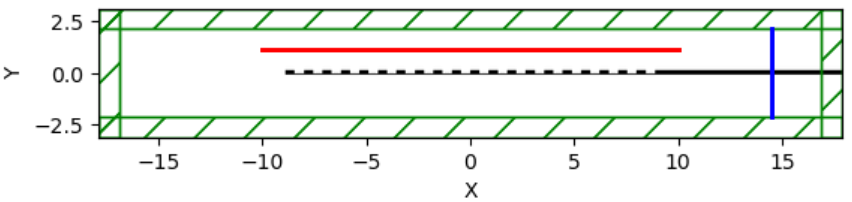
\includegraphics[width=1\linewidth]{Image/geo.png}
    \caption{Geometry of the simulated device ($\mu$m)}
    \label{fig:schema_disp}
\end{figure}

The grating is characterized by its period $\Lambda$ and its duty cycle (fraction of silicon per period). These two parameters are the subject of the optimization presented in chapter~\ref{ch:resultats}. The grating is extended by a single-mode output waveguide, of full thickness, over a length long enough to allow the guided mode to be measured far from any geometric perturbation.

\section{Source modeling}

The incident light is modeled by a Gaussian beam (\texttt{GaussianBeam2DSource} in Meep) rather than an infinite plane wave, in order to faithfully represent the transverse mode profile of a standard single-mode optical fiber. The beam waist radius is set to $w_0=5{,}2$~\textmu m, corresponding to half the mode field diameter (MFD $\approx$10,4~\textmu m) of an SMF-28 fiber at 1550~nm.

The beam is injected at an incidence angle $\theta=10^\circ$ with respect to the normal to the waveguide, a standard choice that avoids part of the reflected light going straight back into the fiber through specular reflection (Fresnel reflection at normal incidence). The beam's focal point is placed at the center of the grating, at a distance of 1~\textmu m above the surface of the waveguide.

The angle of incidence is imposed not by physically orienting the source region (which must necessarily be aligned with the FDTD grid axes), but through the Gaussian beam's propagation-direction parameter (\texttt{beam\_kdir}), which analytically determines the amplitude and phase of the field along the source line so as to reproduce a tilted wavefront.

\section{Physical parameters of the simulations}

Table~\ref{tab:parametres} summarizes all the fixed parameters used to build the geometry and the source in the simulations presented in this report, independently of the grating parameters ($\Lambda$, $gdc$) that are the subject of the optimization.

\begin{table}[h]
\centering
\begin{tabular}{lcl}
\hline
Parameter & Value & Description \\
\hline
$\lambda$ & 1,55~\textmu m & design wavelength \\
$\theta$ & $10^\circ$ & fiber incidence angle \\
$h$ & 0,22~\textmu m & total silicon slab thickness \\
$t_{slab}$ & 0,07~\textmu m & thickness of the non-etched base \\
$t_{etch}$ & 0,15~\textmu m & height of the etched part ($h-t_{slab}$) \\
$N$ & 20 & number of grating teeth \\
$d_{\text{PML}}$ & 1~\textmu m & thickness of the absorbing layers \\
$L_{wg}$ & 8~\textmu m & length of the output waveguide \\
$d_{\text{air}}$ & 2~\textmu m & air margin above/below the slab \\
$w_0$ & 5,2~\textmu m & Gaussian beam waist radius \\
$d_{\text{standoff}}$ & 1~\textmu m & source-to-grating-surface distance \\
resolution & 150~pixels/\textmu m & FDTD spatial resolution used \\
\hline
\end{tabular}
\caption{Fixed physical parameters used in the simulations}
\label{tab:parametres}
\end{table}


%%%%%%%%%%%%%%%%%%%%%%%%%%%%%%%%%% Chapitre 4 : Validation numerique %%%%%%%%%%%%%%%%%%%%%%%%%%%%%%%%%%
\chapter{Numerical validation}
\label{ch:validation}


Before interpreting the optimization results presented in chapter~\ref{ch:resultats}, it is necessary to make sure that the computed efficiency values reflect actual physical behavior and not an artifact of the spatial discretization. This chapter presents the validation process followed, motivated by inconsistencies observed during the first parametric sweeps.

\section{Sensitivity to spatial discretization}

Meep does not discretize material/air interfaces in a binary way (all-or-nothing, pixel by pixel), but instead uses a subpixel-averaging technique: when the edge of a geometric object falls inside a pixel rather than exactly on a grid boundary, an effective permittivity, weighted between the two materials, is assigned to that pixel. This approach in principle achieves a precision finer than the pixel size, even for geometries poorly aligned with the grid.

This technique reduces the discretization error without fully eliminating it: a small residual error remains at each interface. In the case of the grating studied here, this error is repeated at the edges of the $N=20$ teeth, which can lead to a significant accumulation, particularly for a structure with a high index contrast (silicon/air, $\Delta\varepsilon=11$) where this averaging method is known to be less accurate.

A first parametric sweep over the grating period $\Lambda$ revealed this phenomenon: the efficiency values obtained varied non-monotonically and erratically with $\Lambda$, without any physically coherent curve shape. The identified cause is a misalignment between the geometric dimensions (period, tooth width, etch depth) and the computational grid, with each configuration tested falling, in an uncontrolled way, on a different pixel alignment.

\paragraph{Correction: grid alignment (\emph{snapping}).} To eliminate this source of noise, each geometric dimension was systematically rounded to the nearest integer multiple of the pixel size ($1/\text{resolution}$) before the geometry was built:
\begin{equation}
x_{\text{snap}} = \text{round}\left(\frac{x}{\Delta_{\text{pixel}}}\right)\times\Delta_{\text{pixel}}, \qquad \Delta_{\text{pixel}}=\frac{1}{\text{resolution}}
\label{eq:snap}
\end{equation}

This treatment was applied not only to the period $\Lambda$, but also to the grating's origin position and to the thickness of the non-etched base, so that \emph{all} edges of \emph{all} material blocks fall exactly on grid positions. After this correction, the sweep over $\Lambda$ recovered a smooth and monotonic curve shape (figure~\ref{fig:balayage_lambda}), confirming that the initial irregularity was indeed a numerical artifact and not physical behavior.

\section{Resolution convergence study}
\label{sec:convergence}

Once the alignment noise was eliminated, the stability of the results with respect to the spatial resolution itself was checked. The operating point ($\Lambda=0{,}72$~\textmu m, $gdc=0{,}5$) was recomputed at increasing resolution:

\begin{table}[h]
\centering
\begin{tabular}{cc}
\hline
Resolution (pixels/\textmu m) & Efficiency (dB) \\
\hline
50  & $-12,72$ \\
100 & $-16,67$ \\
150 & $-19,29$ \\
\hline
\end{tabular}
\caption{Efficiency at the point $(\Lambda,gdc)=(0{,}72,\,0{,}5)$ as a function of resolution}
\label{tab:convergence}
\end{table}

The discrepancy observed between 50 and 100 pixels/\textmu m (about 4~dB), and again between 100 and 150 pixels/\textmu m (about 2{,}6~dB), indicates that numerical convergence had not yet been fully reached, even at 100~pixels/\textmu m, which is consistent with the sub-wavelength dimensions of the grating elements (teeth on the order of 300~nm, i.e. only 15 to 45 pixels depending on the resolution). A resolution of 150~pixels/\textmu m was retained for all the results presented in chapter~\ref{ch:resultats}, as the best compromise reached between numerical accuracy and computational cost within the time available for the project, the latter growing approximately as the cube of the resolution in two dimensions (two factors linked to spatial refinement, one factor linked to the reduction of the time step imposed by the Courant stability condition) --- with no guarantee that full convergence is reached at this resolution.

%%%%%%%%%%%%%%%%%%%%%%%%%%%%%%%%%% Chapitre 5 : Resultats %%%%%%%%%%%%%%%%%%%%%%%%%%%%%%%%%%
\chapter{Results --- parameter optimization}
\label{ch:resultats}

\section{Optimization of the grating period}
A sweep was carried out manually for different values of the period, around the initial analytical estimate, in order to empirically identify the optimal value. After correcting the discretization artifacts (aligning the geometric dimensions with the FDTD grid) and carrying out the resolution convergence study (section~\ref{sec:convergence}), a resolution of 150~pixels/\textmu m was chosen for this sweep, and the following results were obtained:

\begin{table}[h]
\centering
\begin{tabular}{cc}
\hline
$\Lambda$ (\textmu m) & Efficiency (dB) \\
\hline
0,50 & $-37,73$ \\
0,60 & $-33,17$ \\
0,70 & $-22,86$ \\
0,72 & $-19,29$ \\
0,74 & $-16,75$ \\
0,76 & $-15,84$ \\
0,78 & $-17,52$ \\
0,80 & $-22,79$ \\
0,90 & $-44,53$ \\
\hline
\end{tabular}
\caption{Results of the sweep over the grating period, at fixed $gdc=0{,}5$}
\label{tab:balayage_lambda}
\end{table}

The curve obtained shows a clear bell shape around $\Lambda=0{,}76$~\textmu m (figure~\ref{fig:balayage_lambda}), with a sharp decrease on either side of this peak. This value differs slightly from the optimum identified at a lower resolution (100~pixels/\textmu m, $\Lambda=0{,}72$~\textmu m), confirming that numerical convergence had not yet been fully reached at this intermediate resolution.

The optimal period thus determined, $\Lambda_{opt}=0{,}76$~\textmu m, will be used as the reference for the duty-cycle exploration below and as the starting point for the gradient-based optimization presented in section~\ref{sec:adjoint}.

\begin{figure}[h]
    \centering
    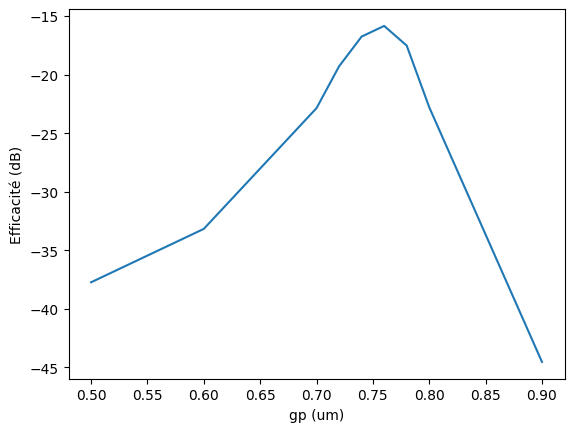
\includegraphics[width=0.7\linewidth]{Image/gp_r150.png}
    \caption{Results of the sweep over the period values, at a resolution of 150~pixels/\textmu m with the duty cycle fixed at 0{,}5}
    \label{fig:balayage_lambda}
\end{figure}


\vspace{0.5em}

\section{Duty-cycle exploration and limitations of the study}
\label{sec:duty_cycle}

A similar sweep was carried out for the duty cycle (proportion of silicon per period), at a fixed period $\Lambda=0{,}72$~\textmu m and a resolution of 150~pixels/\textmu m. The following results were obtained:

\subsection*{Tests on duty-cycle values}
\begin{table}[h]
\centering
\begin{tabular}{cc}
\hline
$gdc$ & Efficiency (dB) \\
\hline
0,40 & $-33,06$ \\
0,50 & $-19,29$ \\
0,60 & $-18,25$ \\
0,65 & $-15,76$ \\
0,67 & $-14,55$ \\
0,69 & $-13,74$ \\
0,70 & $-14,00$ \\
0,71 & $-14,64$ \\
0,73 & $-17,28$ \\
0,75 & $-22,14$ \\
0,80 & $-36,46$ \\
\hline
\end{tabular}
\caption{Results of the sweep over the duty cycle, at fixed $\Lambda=0{,}72$~\textmu m}
\label{tab:balayage_gdc}
\end{table}

\begin{figure}[h]
    \centering
    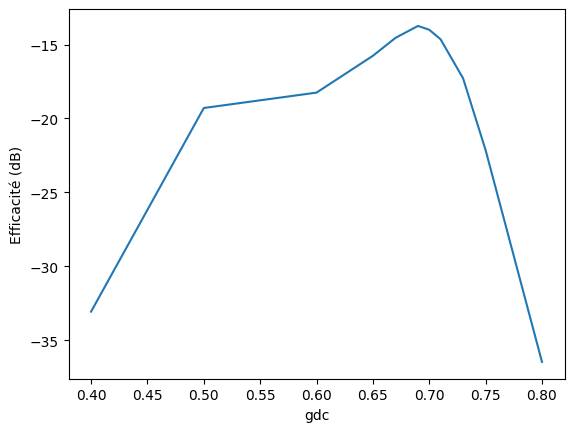
\includegraphics[width=0.7\linewidth]{Image/gdc_r150.png}
    \caption{Results of the sweep over the duty-cycle values, at a resolution of 150~pixels/\textmu m}
    \label{fig:balayage_gdc}
\end{figure}

The curve obtained (figure~\ref{fig:balayage_gdc}) shows a narrow bell shape, with a clear maximum at $gdc=0{,}69$ ($-13{,}74$~dB) and a sharp decrease on either side, particularly beyond $gdc=0{,}73$, where the efficiency drops by more than 20~dB within a few hundredths.

\paragraph{Limitation observed.} This second sweep, carried out at fixed $\Lambda=0{,}72$~\textmu m, gives an optimum ($-13{,}74$~dB at $gdc=0{,}69$) better than the one obtained during the sweep over $\Lambda$ at fixed $gdc=0{,}5$ ($-19{,}29$~dB at the same point $\Lambda=0{,}72$, previous section). This difference confirms that the global optimum of the device does not lie at the values found independently by each of the two sequential sweeps, but in a combination of the two. This motivates the use of a joint optimization of both parameters using the gradient method, presented in section~\ref{sec:adjoint}.


\section{Optimization by gradient ascent}
\label{sec:adjoint}

A gradient-based optimization method was implemented, relying on Meep's built-in adjoint solver to compute the gradient of the coupling efficiency with respect to the two grating parameters ($\Lambda$, $gdc$) simultaneously. For this step, the tilted Gaussian source was temporarily replaced by a simpler, classical source (a plane wave with no tilt), since the adjoint solver proved incompatible with the type of source used for the previous results. The efficiency values reported in this section are therefore not directly comparable, in absolute terms, to those of the manual sweep; the efficiency with the actual source will be recomputed separately, once the optimum has been found.

\subsection*{Starting point close to the manual optimum}

For this optimization, Meep's adjoint solver proved incompatible with the type of source used for the previous results (\texttt{GaussianBeam2DSource}): the gradient computation triggered an internal error, related to how this source is implemented within the adjoint mechanism. The source was therefore replaced by a simple plane wave, to which the incidence angle $\theta=10^\circ$ was reintroduced via a phase function (\texttt{amp\_func}) reproducing the phase shift of a tilted wavefront along the source line. This source preserves the correct phase-matching condition, but does not reproduce the Gaussian transverse profile of the actual beam. 

A trial, starting from the initial conditions $(\Lambda,gdc)=(0{,}7435,\ 0{,}6717)$, a region already identified as favorable by the manual sweep, gives the following results:

\begin{table}[h]
\centering
\begin{tabular}{lcccc}
\hline
Iteration & $\Lambda$ (\textmu m) & $gdc$ & Efficiency (dB) \\
\hline
1 & 0,7435 & 0,6717 & $-18,09$ \\
2 & 0,7525 & 0,6834 & $-16,78$ \\
3 & 0,7612 & 0,6856 & $-15,65$ \\
4 & 0,7590 & 0,6823 & $-10,55$ \\
5 & 0,7596 & 0,6819 & $-10,36$ \\
6 & 0,7652 & 0,6836 & $-12,10$ \\
\hline
\end{tabular}
\caption{Iterations of the gradient optimization (plane wave tilted at $10^\circ$, angle reintroduced via a phase function)}
\label{tab:gradient_iterations}
\end{table}

Despite some residual oscillation, the algorithm progresses consistently toward the optimum of the manual sweep ($gdc\approx0{,}69$, section~\ref{sec:duty_cycle}), reaching $-10{,}36$~dB at iteration 5 with this simplified source, an improvement of nearly 8~dB over the starting point.

\paragraph{Final calculation with the actual source.} The efficiency values above, obtained with the tilted plane wave, are not directly comparable to those of the manual sweep (measured with the actual Gaussian beam). The best point found by the gradient method ($\Lambda=0{,}7596$~\textmu m, $gdc=0{,}6819$) was therefore recomputed with the actual Gaussian source ($w_0=5{,}2$~\textmu m, $\theta=10^\circ$), on the geometry used for the adjoint optimization. This calculation gives an efficiency of $-13{,}39$~dB, a value lower than the $-10{,}36$~dB obtained with the plane wave, but which remains consistent with the optimum of the manual sweep ($-13{,}74$~dB). This discrepancy confirms that the tilted plane wave, although it correctly restores the phase-matching condition, does not reproduce the same coupling physics as an actual Gaussian beam: the optimum found for a uniform illumination of the grating does not exactly correspond to the optimum for a localized beam, whose overlap with the grating's radiation profile depends on parameters not accounted for here.

\section{Comparison of the analytical and numerical models}

Table~\ref{tab:comparaison_finale} summarizes the predictions of the various models developed in chapter~\ref{ch:theorie}, compared against the numerical results obtained through the manual sweep and then through gradient optimization.

\begin{table}[h]
\centering
\begin{tabular}{lccc}
\hline
Method & $\Lambda$ (nm) & $gdc$ & Efficiency (dB) \\
\hline
Volumetric weighting (analytical) & 762 & 0,50 (fixed) & --- \\
Multilayer model (analytical) & 758 & 0,50 (fixed) & --- \\
Manual sweep (FDTD, actual source) & 720 & 0,69 (optimized) & $-13,74$ \\
Gradient optimization (FDTD, actual source) & 759,6 & 0,6819 (optimized) & $-13,39$ \\
\hline
\end{tabular}
\caption{Comparison of the periods predicted by the analytical models and the numerical results}
\label{tab:comparaison_finale}
\end{table}

The two analytical models, evaluated at $gdc=0{,}5$ (a value fixed as input, not optimized by these models), predict a period very close to the FDTD optimum, confirming that a good part of the phase-matching physics is already captured without a full FDTD simulation. This comparison, however, only concerns the period: these analytical models provide no indication of the optimal duty-cycle value itself, which only the FDTD sweep and the gradient optimization were able to identify.

The gradient optimization, once its result is recomputed with the Gaussian source, converges to an efficiency ($-13{,}39$~dB) very close to that of the manual sweep ($-13{,}74$~dB), at a slightly different point ($\Lambda=759{,}6$~nm, $gdc=0{,}6819$ versus $720$~nm, $0{,}69$). 

\section{Adding a bottom reflector}

\subsection*{Problem statement}

In the geometry studied so far, the medium below the grating is symmetric to the upper cladding (air), so half of the power diffracted downward is lost. We therefore decided to study the addition of a buried-oxide layer (BOX, index $n_{BOX}\approx1{,}44$) between the silicon and the substrate, whose thickness $t_{BOX}$ is chosen to redirect this light upward through constructive interference, rather than letting it be transmitted into the substrate.
This gives the following schematic:
\begin{figure}[H]
    \centering
    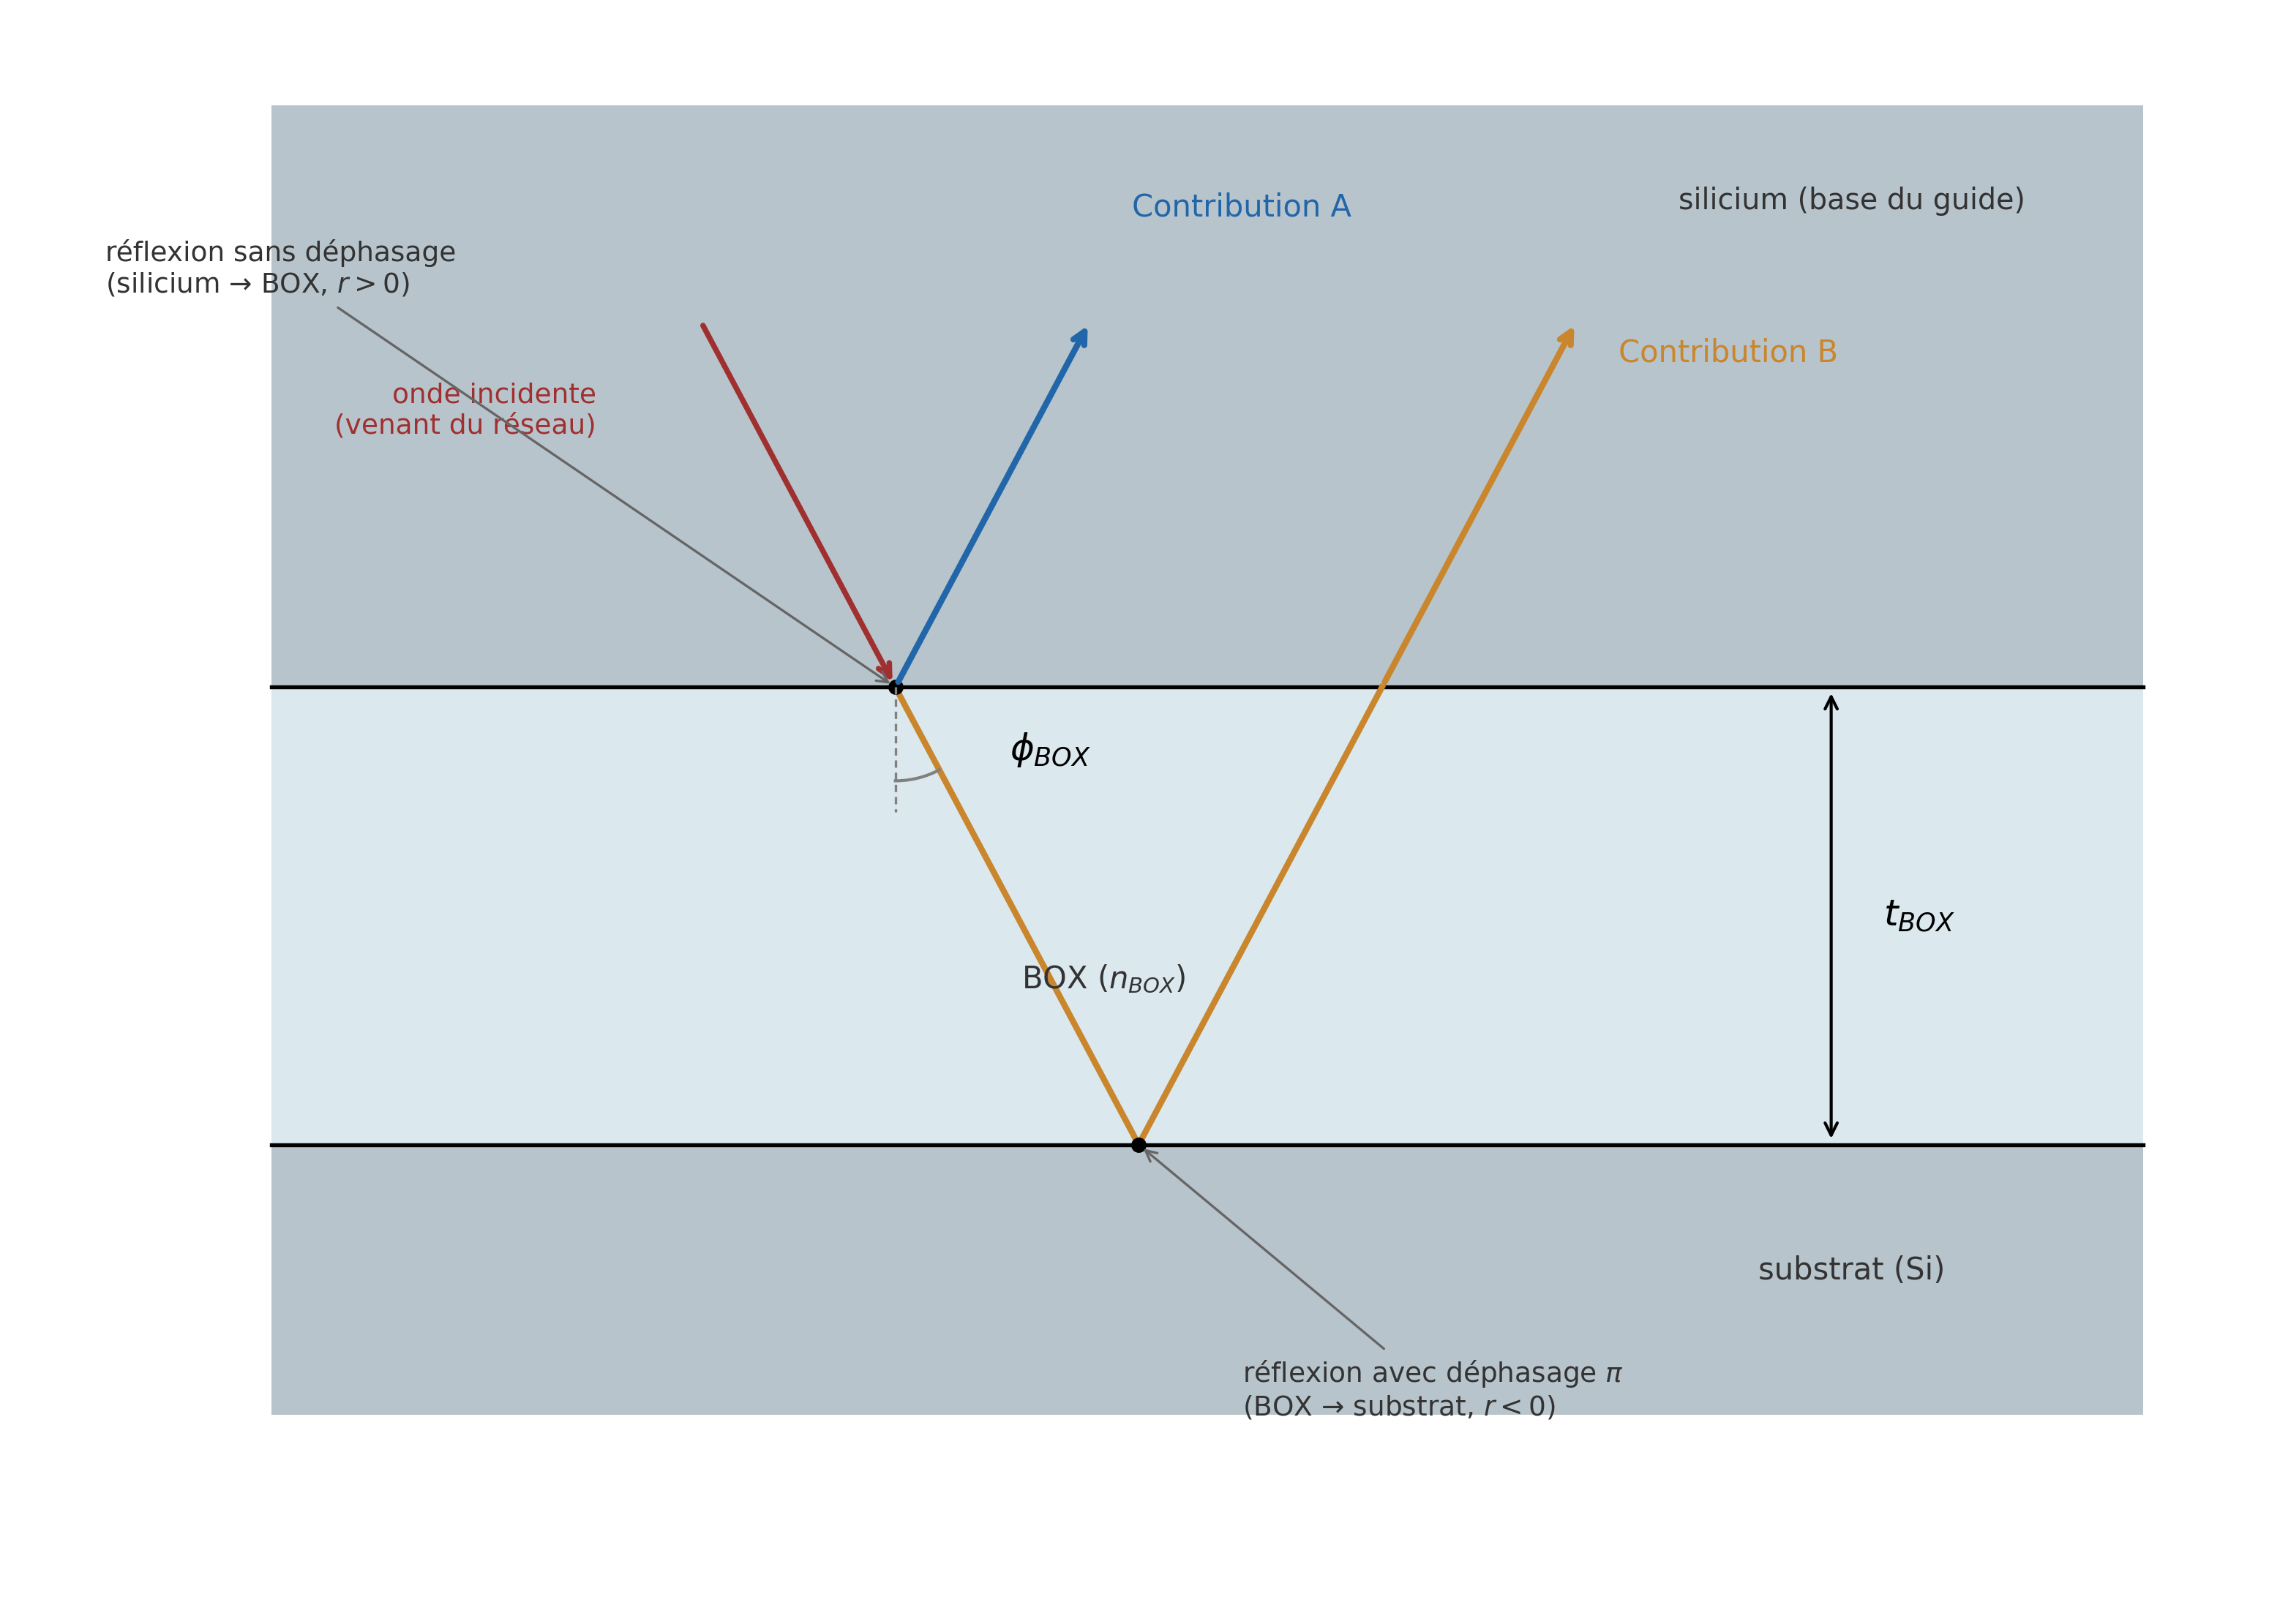
\includegraphics[width=1\linewidth]{Image/schema_box_diff_marche.png}
    \caption{Paths of contributions A and B for the path-difference calculation in the BOX reflector}
    \label{fig:box_diff_marche}
\end{figure}
\begin{itemize}
    \item \textbf{Contribution A}: direct reflection at the first interface (silicon~$\rightarrow$~BOX);
    \item \textbf{Contribution B}: transmission into the BOX, reflection at the second interface (BOX~$\rightarrow$~substrate), then return through the BOX.
\end{itemize}

\subsection*{Phase shift upon reflection}

According to Fresnel's equations at normal incidence, the reflection coefficient at an interface between a medium of index $n_1$ (incident) and a medium of index $n_2$ (transmitted) is written $r=(n_1-n_2)/(n_1+n_2)$. Its sign determines a phase shift of either $0$ or $\pi$:

\begin{itemize}
    \item \textbf{Interface silicon~$\rightarrow$~BOX} ($n_1=n_{Si}>n_2=n_{BOX}$): $r_1>0$, no additional phase shift upon reflection (contribution A);
    \item \textbf{Interface BOX~$\rightarrow$~substrate} ($n_1=n_{BOX}<n_2=n_{Si}$): $r_2<0$, which corresponds to an additional phase shift of $\pi$ upon reflection (contribution B).
\end{itemize}

\subsection*{Path difference and constructive interference condition}

The light diffracted by the grating reaches the BOX at an angle $\phi_{BOX}$ with respect to the normal. Contribution B travels, relative to contribution A, an additional optical distance corresponding to the round trip inside the BOX layer. We thus have the following expression:
\begin{equation}
\delta_{BOX} = \frac{2\,n_{BOX}\,t_{BOX}}{\cos\phi_{BOX}}
\end{equation}
This gives a phase shift equal to:
\begin{equation}
\Delta\varphi = \dfrac{2\pi}{\lambda}\,\delta_{BOX} = \dfrac{4\pi\,n_{BOX}\,t_{BOX}}{\lambda\cos\phi_{BOX}}
\end{equation}
Taking into account the additional phase shift of $\pi$ experienced by contribution B upon its reflection (and not by contribution A), the total phase shift between the two contributions is:
\begin{equation}
\Delta\varphi = \frac{4\pi\,n_{BOX}\,t_{BOX}}{\lambda\cos\phi_{BOX}} + \pi
\end{equation}
For the two contributions to interfere constructively, this phase shift must be an integer multiple of 2$\pi$:
\begin{equation}
\Delta\varphi = 2m\pi, \qquad m\in\mathbb{N}^*
\end{equation}
We therefore have:
\begin{equation}
\frac{4\pi\,n_{BOX}\,t_{BOX}}{\lambda\cos\phi_{BOX}} = (2m-1)\pi
\end{equation}
Thus:
\begin{equation}
\boxed{t_{BOX} = \frac{(2m-1)\,\lambda\,\cos\phi_{BOX}}{4\,n_{BOX}}}
\label{eq:box_quarter_wave}
\end{equation}

\subsection*{Numerical result}

With $\lambda=1{,}55$~\textmu m and $n_{BOX}=1{,}44$ (and a zero incidence angle), the first candidate thicknesses are:
\begin{equation}
t_{BOX}\approx0{,}269~\text{\textmu m}\ (m=1), \quad 0{,}807~\text{\textmu m}\ (m=2), \quad 1{,}345~\text{\textmu m}\ (m=3)
\end{equation}
These values serve as the starting point for an FDTD sweep, with the geometry and grating parameters ($\Lambda$, $gdc$) kept fixed at the previously determined optimum.

\paragraph{Result.}The sweep carried out (thicknesses from 0{,}03 to 1{,}0~\textmu m) did not identify a BOX thickness that improves the efficiency compared to the geometry without a reflector ($-13{,}39$~dB). All the values tested give a lower result, with a local maximum at $-15{,}97$~dB for $t_{BOX}=0{,}06$~\textmu m. This result suggests that the simplified two-wave model (interference between the first two reflections) used for the analytical estimate is insufficient. The thin layer sandwiched between two silicon media in fact appears to form a Fabry-Pérot cavity with multiple reflections, whose behavior is difficult to predict. A more in-depth theoretical study would be needed to draw conclusions on the potential of this reflector; however, this could not be carried out within the time available for this project. 

Table~\ref{tab:box_balayage} presents the results of the sweep over the BOX thickness, with $\Lambda$ and $gdc$ fixed at the previously determined optimum.
\begin{table}[h]
\centering
\begin{tabular}{cc}
\hline
$t_{BOX}$ (\textmu m) & Efficiency (dB) \\
\hline
--- (no BOX, reference) & $-13,39$ \\
0,030 & $-25,93$ \\
0,060 & $-15,97$ \\
0,090 & $-17,33$ \\
0,120 & $-19,63$ \\
0,150 & $-20,80$ \\
0,200 & $-26,24$ \\
0,270 & $-33,52$ \\
0,350 & $-31,46$ \\
0,450 & $-30,07$ \\
0,600 & $-23,13$ \\
0,807 & $-37,01$ \\
1,000 & $-25,28$ \\
\hline
\end{tabular}
\caption{Results of the sweep over the BOX reflector thickness, with $\Lambda$ and $gdc$ fixed at the optimum}
\label{tab:box_balayage}
\end{table}

\chapter{Conclusion}

\section{Summary}

This project aimed to design, simulate, and optimize a silicon fiber-to-chip grating coupler, combining an analytical approach with an FDTD simulation under Meep. The approach followed a coherent progression: an initial theoretical estimate of the grating period, progressively refined by analytical models increasingly faithful to the actual geometry (volumetric weighting, then a multilayer transfer-matrix model); a rigorous numerical implementation, validated by a study of the sensitivity to spatial discretization and of resolution convergence; then an optimization of the grating parameters, carried out both through a manual parametric sweep and through a gradient method relying on Meep's adjoint solver.

The two most advanced analytical models predict a period of $758$ to $762$~nm, very close to the numerically identified optimum ($760$~nm), confirming that a significant part of the coupling physics (constructive interference condition) is correctly captured by a simplified effective-index model, without requiring a full simulation. Optimization of the two grating parameters ($\Lambda$, $gdc$), carried out through manual sweeping and then through the gradient method, achieved a coupling efficiency of $-13{,}4$~dB (about $4{,}6\%$), with both methods converging to points very close to each other in parameter space.

\section{Limitations of the study}

Several limitations were identified over the course of the project, explaining the gap between the efficiency obtained and the values typically seen in publications on this type of component (typically $-1$ to $-3$~dB):

\begin{itemize}
    \item \textbf{Absence of an effective bottom reflector.} The addition of a buried-oxide layer (BOX), meant to redirect toward the fiber half of the power diffracted toward the substrate, did not yield any improvement in the sweep carried out. This result is explained by the limitation of the analytical model used, a two-wave approximation, whereas the structure in reality forms a Fabry-Pérot cavity with many more, and more complex, reflections.
    \item \textbf{Uniform, non-apodized grating.} Even in the ideal case, a grating with identical teeth cannot perfectly match the Gaussian profile of the incident beam, which therefore reduces the final measured efficiency.
    \item \textbf{Partially joint optimization.} Only two geometric parameters ($\Lambda$, $gdc$) were optimized, out of the five or six that actually influence the efficiency (etch depth, focal-point position, number of teeth, BOX thickness).
    \item \textbf{Gaussian source incompatible with gradient optimization.} Meep's adjoint solver proved incompatible with the Gaussian-beam source used for the reference results. The source had to be simplified (plane wave, then plane wave tilted via a phase function) for this step, requiring a final recalculation to obtain a result comparable to the other methods.
    \item \textbf{Two-dimensional modeling.} The entire study relies on a 2D approximation, which ignores the actual lateral confinement of a finite-width waveguide and the associated losses.
\end{itemize}

\section{Future work}

Several avenues, identified but not explored within the time available for this project, would significantly improve the efficiency obtained:

\begin{itemize}
    \item varying the etch depth and the duty cycle along the grating (apodization) to better match the Gaussian profile of the incident beam;
    \item a more rigorous modeling of the BOX reflector, accounting for multiple reflections;
    \item a better adjoint-gradient optimization, which would allow more complex grating geometries to be explored.
\end{itemize}
\end{document}